% Generated by Sphinx.
\def\sphinxdocclass{report}
\documentclass[letterpaper,10pt,english]{sphinxmanual}
\usepackage[utf8]{inputenc}
\DeclareUnicodeCharacter{00A0}{\nobreakspace}
\usepackage{cmap}
\usepackage[T1]{fontenc}
\usepackage{babel}
\usepackage{times}
\usepackage[Bjarne]{fncychap}
\usepackage{longtable}
\usepackage{sphinx}
\usepackage{multirow}


\title{JFORTES Documentation}
\date{October 01, 2014}
\release{1}
\author{Herbert Rocha}
\newcommand{\sphinxlogo}{}
\renewcommand{\releasename}{Release}
\makeindex

\makeatletter
\def\PYG@reset{\let\PYG@it=\relax \let\PYG@bf=\relax%
    \let\PYG@ul=\relax \let\PYG@tc=\relax%
    \let\PYG@bc=\relax \let\PYG@ff=\relax}
\def\PYG@tok#1{\csname PYG@tok@#1\endcsname}
\def\PYG@toks#1+{\ifx\relax#1\empty\else%
    \PYG@tok{#1}\expandafter\PYG@toks\fi}
\def\PYG@do#1{\PYG@bc{\PYG@tc{\PYG@ul{%
    \PYG@it{\PYG@bf{\PYG@ff{#1}}}}}}}
\def\PYG#1#2{\PYG@reset\PYG@toks#1+\relax+\PYG@do{#2}}

\expandafter\def\csname PYG@tok@gd\endcsname{\def\PYG@tc##1{\textcolor[rgb]{0.63,0.00,0.00}{##1}}}
\expandafter\def\csname PYG@tok@gu\endcsname{\let\PYG@bf=\textbf\def\PYG@tc##1{\textcolor[rgb]{0.50,0.00,0.50}{##1}}}
\expandafter\def\csname PYG@tok@gt\endcsname{\def\PYG@tc##1{\textcolor[rgb]{0.00,0.27,0.87}{##1}}}
\expandafter\def\csname PYG@tok@gs\endcsname{\let\PYG@bf=\textbf}
\expandafter\def\csname PYG@tok@gr\endcsname{\def\PYG@tc##1{\textcolor[rgb]{1.00,0.00,0.00}{##1}}}
\expandafter\def\csname PYG@tok@cm\endcsname{\let\PYG@it=\textit\def\PYG@tc##1{\textcolor[rgb]{0.25,0.50,0.56}{##1}}}
\expandafter\def\csname PYG@tok@vg\endcsname{\def\PYG@tc##1{\textcolor[rgb]{0.73,0.38,0.84}{##1}}}
\expandafter\def\csname PYG@tok@m\endcsname{\def\PYG@tc##1{\textcolor[rgb]{0.13,0.50,0.31}{##1}}}
\expandafter\def\csname PYG@tok@mh\endcsname{\def\PYG@tc##1{\textcolor[rgb]{0.13,0.50,0.31}{##1}}}
\expandafter\def\csname PYG@tok@cs\endcsname{\def\PYG@tc##1{\textcolor[rgb]{0.25,0.50,0.56}{##1}}\def\PYG@bc##1{\setlength{\fboxsep}{0pt}\colorbox[rgb]{1.00,0.94,0.94}{\strut ##1}}}
\expandafter\def\csname PYG@tok@ge\endcsname{\let\PYG@it=\textit}
\expandafter\def\csname PYG@tok@vc\endcsname{\def\PYG@tc##1{\textcolor[rgb]{0.73,0.38,0.84}{##1}}}
\expandafter\def\csname PYG@tok@il\endcsname{\def\PYG@tc##1{\textcolor[rgb]{0.13,0.50,0.31}{##1}}}
\expandafter\def\csname PYG@tok@go\endcsname{\def\PYG@tc##1{\textcolor[rgb]{0.20,0.20,0.20}{##1}}}
\expandafter\def\csname PYG@tok@cp\endcsname{\def\PYG@tc##1{\textcolor[rgb]{0.00,0.44,0.13}{##1}}}
\expandafter\def\csname PYG@tok@gi\endcsname{\def\PYG@tc##1{\textcolor[rgb]{0.00,0.63,0.00}{##1}}}
\expandafter\def\csname PYG@tok@gh\endcsname{\let\PYG@bf=\textbf\def\PYG@tc##1{\textcolor[rgb]{0.00,0.00,0.50}{##1}}}
\expandafter\def\csname PYG@tok@ni\endcsname{\let\PYG@bf=\textbf\def\PYG@tc##1{\textcolor[rgb]{0.84,0.33,0.22}{##1}}}
\expandafter\def\csname PYG@tok@nl\endcsname{\let\PYG@bf=\textbf\def\PYG@tc##1{\textcolor[rgb]{0.00,0.13,0.44}{##1}}}
\expandafter\def\csname PYG@tok@nn\endcsname{\let\PYG@bf=\textbf\def\PYG@tc##1{\textcolor[rgb]{0.05,0.52,0.71}{##1}}}
\expandafter\def\csname PYG@tok@no\endcsname{\def\PYG@tc##1{\textcolor[rgb]{0.38,0.68,0.84}{##1}}}
\expandafter\def\csname PYG@tok@na\endcsname{\def\PYG@tc##1{\textcolor[rgb]{0.25,0.44,0.63}{##1}}}
\expandafter\def\csname PYG@tok@nb\endcsname{\def\PYG@tc##1{\textcolor[rgb]{0.00,0.44,0.13}{##1}}}
\expandafter\def\csname PYG@tok@nc\endcsname{\let\PYG@bf=\textbf\def\PYG@tc##1{\textcolor[rgb]{0.05,0.52,0.71}{##1}}}
\expandafter\def\csname PYG@tok@nd\endcsname{\let\PYG@bf=\textbf\def\PYG@tc##1{\textcolor[rgb]{0.33,0.33,0.33}{##1}}}
\expandafter\def\csname PYG@tok@ne\endcsname{\def\PYG@tc##1{\textcolor[rgb]{0.00,0.44,0.13}{##1}}}
\expandafter\def\csname PYG@tok@nf\endcsname{\def\PYG@tc##1{\textcolor[rgb]{0.02,0.16,0.49}{##1}}}
\expandafter\def\csname PYG@tok@si\endcsname{\let\PYG@it=\textit\def\PYG@tc##1{\textcolor[rgb]{0.44,0.63,0.82}{##1}}}
\expandafter\def\csname PYG@tok@s2\endcsname{\def\PYG@tc##1{\textcolor[rgb]{0.25,0.44,0.63}{##1}}}
\expandafter\def\csname PYG@tok@vi\endcsname{\def\PYG@tc##1{\textcolor[rgb]{0.73,0.38,0.84}{##1}}}
\expandafter\def\csname PYG@tok@nt\endcsname{\let\PYG@bf=\textbf\def\PYG@tc##1{\textcolor[rgb]{0.02,0.16,0.45}{##1}}}
\expandafter\def\csname PYG@tok@nv\endcsname{\def\PYG@tc##1{\textcolor[rgb]{0.73,0.38,0.84}{##1}}}
\expandafter\def\csname PYG@tok@s1\endcsname{\def\PYG@tc##1{\textcolor[rgb]{0.25,0.44,0.63}{##1}}}
\expandafter\def\csname PYG@tok@gp\endcsname{\let\PYG@bf=\textbf\def\PYG@tc##1{\textcolor[rgb]{0.78,0.36,0.04}{##1}}}
\expandafter\def\csname PYG@tok@sh\endcsname{\def\PYG@tc##1{\textcolor[rgb]{0.25,0.44,0.63}{##1}}}
\expandafter\def\csname PYG@tok@ow\endcsname{\let\PYG@bf=\textbf\def\PYG@tc##1{\textcolor[rgb]{0.00,0.44,0.13}{##1}}}
\expandafter\def\csname PYG@tok@sx\endcsname{\def\PYG@tc##1{\textcolor[rgb]{0.78,0.36,0.04}{##1}}}
\expandafter\def\csname PYG@tok@bp\endcsname{\def\PYG@tc##1{\textcolor[rgb]{0.00,0.44,0.13}{##1}}}
\expandafter\def\csname PYG@tok@c1\endcsname{\let\PYG@it=\textit\def\PYG@tc##1{\textcolor[rgb]{0.25,0.50,0.56}{##1}}}
\expandafter\def\csname PYG@tok@kc\endcsname{\let\PYG@bf=\textbf\def\PYG@tc##1{\textcolor[rgb]{0.00,0.44,0.13}{##1}}}
\expandafter\def\csname PYG@tok@c\endcsname{\let\PYG@it=\textit\def\PYG@tc##1{\textcolor[rgb]{0.25,0.50,0.56}{##1}}}
\expandafter\def\csname PYG@tok@mf\endcsname{\def\PYG@tc##1{\textcolor[rgb]{0.13,0.50,0.31}{##1}}}
\expandafter\def\csname PYG@tok@err\endcsname{\def\PYG@bc##1{\setlength{\fboxsep}{0pt}\fcolorbox[rgb]{1.00,0.00,0.00}{1,1,1}{\strut ##1}}}
\expandafter\def\csname PYG@tok@kd\endcsname{\let\PYG@bf=\textbf\def\PYG@tc##1{\textcolor[rgb]{0.00,0.44,0.13}{##1}}}
\expandafter\def\csname PYG@tok@ss\endcsname{\def\PYG@tc##1{\textcolor[rgb]{0.32,0.47,0.09}{##1}}}
\expandafter\def\csname PYG@tok@sr\endcsname{\def\PYG@tc##1{\textcolor[rgb]{0.14,0.33,0.53}{##1}}}
\expandafter\def\csname PYG@tok@mo\endcsname{\def\PYG@tc##1{\textcolor[rgb]{0.13,0.50,0.31}{##1}}}
\expandafter\def\csname PYG@tok@mi\endcsname{\def\PYG@tc##1{\textcolor[rgb]{0.13,0.50,0.31}{##1}}}
\expandafter\def\csname PYG@tok@kn\endcsname{\let\PYG@bf=\textbf\def\PYG@tc##1{\textcolor[rgb]{0.00,0.44,0.13}{##1}}}
\expandafter\def\csname PYG@tok@o\endcsname{\def\PYG@tc##1{\textcolor[rgb]{0.40,0.40,0.40}{##1}}}
\expandafter\def\csname PYG@tok@kr\endcsname{\let\PYG@bf=\textbf\def\PYG@tc##1{\textcolor[rgb]{0.00,0.44,0.13}{##1}}}
\expandafter\def\csname PYG@tok@s\endcsname{\def\PYG@tc##1{\textcolor[rgb]{0.25,0.44,0.63}{##1}}}
\expandafter\def\csname PYG@tok@kp\endcsname{\def\PYG@tc##1{\textcolor[rgb]{0.00,0.44,0.13}{##1}}}
\expandafter\def\csname PYG@tok@w\endcsname{\def\PYG@tc##1{\textcolor[rgb]{0.73,0.73,0.73}{##1}}}
\expandafter\def\csname PYG@tok@kt\endcsname{\def\PYG@tc##1{\textcolor[rgb]{0.56,0.13,0.00}{##1}}}
\expandafter\def\csname PYG@tok@sc\endcsname{\def\PYG@tc##1{\textcolor[rgb]{0.25,0.44,0.63}{##1}}}
\expandafter\def\csname PYG@tok@sb\endcsname{\def\PYG@tc##1{\textcolor[rgb]{0.25,0.44,0.63}{##1}}}
\expandafter\def\csname PYG@tok@k\endcsname{\let\PYG@bf=\textbf\def\PYG@tc##1{\textcolor[rgb]{0.00,0.44,0.13}{##1}}}
\expandafter\def\csname PYG@tok@se\endcsname{\let\PYG@bf=\textbf\def\PYG@tc##1{\textcolor[rgb]{0.25,0.44,0.63}{##1}}}
\expandafter\def\csname PYG@tok@sd\endcsname{\let\PYG@it=\textit\def\PYG@tc##1{\textcolor[rgb]{0.25,0.44,0.63}{##1}}}

\def\PYGZbs{\char`\\}
\def\PYGZus{\char`\_}
\def\PYGZob{\char`\{}
\def\PYGZcb{\char`\}}
\def\PYGZca{\char`\^}
\def\PYGZam{\char`\&}
\def\PYGZlt{\char`\<}
\def\PYGZgt{\char`\>}
\def\PYGZsh{\char`\#}
\def\PYGZpc{\char`\%}
\def\PYGZdl{\char`\$}
\def\PYGZhy{\char`\-}
\def\PYGZsq{\char`\'}
\def\PYGZdq{\char`\"}
\def\PYGZti{\char`\~}
% for compatibility with earlier versions
\def\PYGZat{@}
\def\PYGZlb{[}
\def\PYGZrb{]}
\makeatother

\renewcommand\PYGZsq{\textquotesingle}

\begin{document}

\maketitle
\tableofcontents
\phantomsection\label{index::doc}


Contents:


\chapter{Introduction to JFORTES}
\label{sections/intro:introduction-to-jfortes}\label{sections/intro:welcome-to-jfortes-s-documentation}\label{sections/intro::doc}
Nowadays, software applications need to be developed quickly and meet a high-level
of quality. Formal verification plays an important role to ensure predictability and dependability
in the design of critical applications. Consequently, the application of verification and testing are
indispensable techniques to the development of high-quality
software. However, there is usually a high cost involved in the preparation, execution
and management of tests. One way to deal with such problems is to integrate formal verification
techniques with test environments \footnote{
Herbert Rocha, Lucas Cordeiro, Raimundo Barreto and José Netto. Exploiting Safety Properties in Bounded Model
Checking for Test Cases Generation of C Programs. In SAST. SBC. 2010.
}.

JFORTES  (Java FORmal unit TESt generation) is a method that aims to extract the safety properties generated
by ESC/JAVA \footnote{
Available at \href{http://kindsoftware.com/products/opensource/ESCJava2/}{http://kindsoftware.com/products/opensource/ESCJava2/}
} to generate automatically test cases using the rich set of assertions provided by Unit Test
frameworks, such as: TestNG \footnote{
Available at \href{http://testng.org/doc/index.html}{http://testng.org/doc/index.html}
} and JCUTE \footnote{
Available at \href{http://osl.cs.illinois.edu/software/jcute/}{http://osl.cs.illinois.edu/software/jcute/}
} . The integration of these two environments aims to ensure software
quality by exploiting formal verification and tests. JFORTES is a extension of FORTES \footnote{
Available at \href{https://sites.google.com/site/fortesmethod/}{https://sites.google.com/site/fortesmethod/}
} to Java programs.
{\hyperref[sections/intro:fig-flow-jfortes]{\emph{Figure 1: JFORTES Flow}}} shows a flow structure of the JFORTES method.
We advocate that exploiting the integration between a testing framework and formal verification allows
us to go deeper into the Java program verification.
\begin{figure}[htbp]
\centering
\capstart

\scalebox{1.000000}{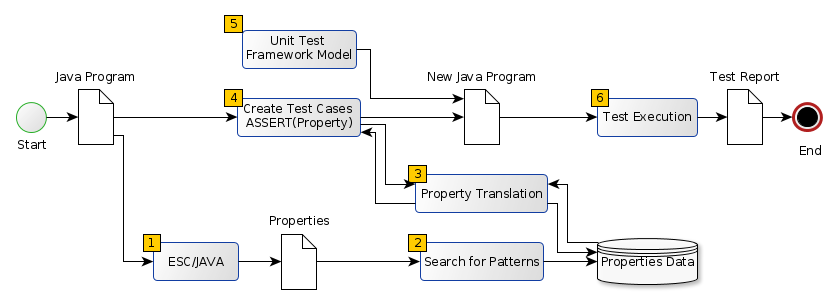
\includegraphics{jfortes_flow.png}}
\caption{Figure 1: JFORTES Flow}\label{sections/intro:fig-flow-jfortes}\end{figure}
\paragraph{References}


\chapter{JFORTES's Tutorial}
\label{sections/tutorial::doc}\label{sections/tutorial:jfortes-s-tutorial}
JFORTES aims to extract the safety properties generated by ESC/JAVA \footnote{
Available at \href{http://kindsoftware.com/products/opensource/ESCJava2/}{http://kindsoftware.com/products/opensource/ESCJava2/}
} to generate automatically
test cases using the rich set of assertions provided by Unit Test frameworks.


\section{Requirements for using the tool}
\label{sections/tutorial:requirements-for-using-the-tool}
To use this tool is necessary that the system contains the following software already installed properly:
\begin{itemize}
\item {} 
Python

\item {} 
ESC/JAVA \footnotemark[1]

\item {} 
Java 1.5 \footnote{
Available at \href{http://www.oracle.com/technetwork/java/javasebusiness/downloads/java-archive-downloads-javase5-419410.html}{http://www.oracle.com/technetwork/java/javasebusiness/downloads/java-archive-downloads-javase5-419410.html}
}

\item {} 
Ctags \footnote{
Available at \href{http://ctags.sourceforge.net/}{http://ctags.sourceforge.net/}
}

\end{itemize}

WARNNING: ESC/Java2 is written with Java 1.4 and only runs in a Java 1.4 or 1.5 virtual machine.
While ESC/Java2 should work in any Java 1.4 or 1.5 virtual machine.


\section{How to install JFortes?}
\label{sections/tutorial:how-to-install-jfortes}
In order to install JFortes on your PC, you should download and save the JFORTES\_vx.zip file on your disk.
After that, you should type the following command:


\subsection{STEP 1:}
\label{sections/tutorial:step-1}
\begin{Verbatim}[commandchars=\\\{\}]
\PYG{n+nv}{\PYGZdl{} }tar \PYGZhy{}xzvf JFORTES\PYGZus{}vx.zip
\end{Verbatim}

or from GITHUB

\begin{Verbatim}[commandchars=\\\{\}]
\PYG{n+nv}{\PYGZdl{} }git clone https://github.com/hbgit/jfortes.git
\end{Verbatim}


\subsection{STEP 2:}
\label{sections/tutorial:step-2}
Open the directory where the JFortes tool was extracted and then you should locate the configure.py script.
After that, you should run the configure.py script, it is worth to say that you should run the configure.py script
from inside the directory where JFortes was extracted.

\begin{Verbatim}[commandchars=\\\{\}]
\PYG{n+nv}{\PYGZdl{} }\PYG{n+nb}{cd }JFortes\PYGZus{}vx
\PYG{n+nv}{\PYGZdl{} }ls
\PYG{n+nv}{\PYGZdl{} }./configure.py
\end{Verbatim}

Now it is advisable that you should set the environment variable PATH in your .bashrc for:
\begin{itemize}
\item {} 
Java 5

\end{itemize}

\begin{Verbatim}[commandchars=\\\{\}]
\PYG{c}{\PYGZsh{} \PYGZhy{}\PYGZhy{}\PYGZhy{} Java 5}
\PYG{n+nv}{\PYGZdl{} }\PYG{n+nv}{JAVA\PYGZus{}HOME}\PYG{o}{=}\PYG{l+s+s2}{\PYGZdq{}/usr/lib/java/jdk1.5.0\PYGZus{}22/\PYGZdq{}}
\PYG{n+nv}{\PYGZdl{} }\PYG{n+nb}{export }JAVA\PYGZus{}HOME
\PYG{n+nv}{\PYGZdl{} }\PYG{n+nb}{export }\PYG{n+nv}{PATH}\PYG{o}{=}\PYG{n+nv}{\PYGZdl{}JAVA\PYGZus{}HOME}/bin:\PYG{n+nv}{\PYGZdl{}PATH}
\end{Verbatim}
\begin{itemize}
\item {} 
ESC/JAVA

\end{itemize}

\begin{Verbatim}[commandchars=\\\{\}]
\PYG{n+nb}{export }\PYG{n+nv}{PATH}\PYG{o}{=}\PYG{n+nv}{\PYGZdl{}PATH}:/home/hrocha/Downloads/ESCJava\PYGZhy{}2.0.5\PYGZhy{}04\PYGZhy{}11\PYGZhy{}08\PYGZhy{}binary/
\end{Verbatim}


\subsection{STEP 3:}
\label{sections/tutorial:step-3}
It is advisable that you should set the environment variable PATH in your .bashrc file as follows:

\begin{Verbatim}[commandchars=\\\{\}]
\PYG{n+nv}{\PYGZdl{} }\PYG{n+nb}{export }\PYG{n+nv}{PATH}\PYG{o}{=}\PYG{n+nv}{\PYGZdl{}PATH}:/home/user/JFortes\PYGZus{}vx/
\end{Verbatim}


\subsection{STEP 4:}
\label{sections/tutorial:step-4}
Testing Map2Check-Fortes

\begin{Verbatim}[commandchars=\\\{\}]
\PYG{n+nv}{\PYGZdl{} }jfortes.py test\PYGZus{}cases/primary\PYGZus{}tests/Bag.java
\end{Verbatim}
\paragraph{References}


\chapter{JFORTES's Limitations}
\label{sections/limitations:jfortes-s-limitations}\label{sections/limitations::doc}
DOING...


\chapter{Indices and tables}
\label{index:indices-and-tables}\begin{itemize}
\item {} 
\emph{genindex}

\item {} 
\emph{modindex}

\item {} 
\emph{search}

\end{itemize}



\renewcommand{\indexname}{Index}
\printindex
\end{document}
